\scanpage{33}
\mspage{32}

% L1–2
1) For the order relation, there is a least element $\varnothing$, and a greatest element $L$ \inserted{(or $1$)}.

% L3
2) : $X\subset Y\Rightarrow\{X,Y\}$ tame

% L4
3) If $\{X,Y\}$ tame, $X\wedge Y$ and $X\vee Y$ exist (infimum and supremum)
% Lleft, opposite 3
% slanted
\margin{- Caution $X\vee Y$ \deleted{\unsure{is|not}} is \uline{not} the union \deleted{of} $X\cup Y$ !!}

% L5–6
\deleted{\unsure{3)|3 bis)} If $\{X,\unsure{Y_i|Y}\}$ \unsure{is|are} \illegible{2} tame, then} \deleted{If \unsure{two|the} $X$ \unsure{and|are} \unsure{tame} \unsure{for}} \inserted{(distributivity) and for a family of mutuall\textsuperscript{y} tame \unsure{elements|elements}, $X\wedge(\bigvee_iY_i)=\bigvee_i(X\wedge Y_i)$}

% L7–11
\deleted{\unsure{3|5}}4) \deleted{Among the} $\forall X\in\mathcal M$ \deleted{\unsure{elements|there exists}}, \deleted{\unsure{in|of the}} among the $Y\in\mathcal M$ such that $\{X,Y\}$ tame, and $X\wedge Y=\varnothing$, there is a greatest element \inserted{$X'$}. It is also the unique element such that
% Lleft, opposite X′ and tel que
% slanted
\margin{\uline{Say also} If \deleted{\unsure{(element)|($X_i$)}} $\{X_i\}_{i\in\unsure{I|J}}\subset\mathcal M$ is formed of \unsure{mutually|mutually} tame elemen\textsuperscript{ts}, then for the operations $\wedge,\vee,'$ they generate a ``Boolean algebra'', finite if $I$ finite.\figure{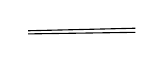
\begin{tikzpicture}[x=.4cm,y=.4cm]\draw (0,0)--(3.4,.08);\draw (0,-.1)--(3.4,-.05);\end{tikzpicture}}}
% L12
\[
\{X',X\}\text{ tame},\qquad \unsure{X''|X'}\wedge X=\varnothing,\qquad X'\vee X=1
\]
% L13–17
Thus the map $X\mapsto X'$ is involutive, it reverses the order relation (anti-involution), \deleted{thus interchanges} \deleted{\unsure{Of|One}}Moreover $\{X\ \mathrm{and}\ Y\}$ are tame if and only if $\{X',Y'\}$ tame\textsuperscript{*},
% Lleft of same passage
% slanted
\margin{* In fact, $\forall X,Y$ $\{X,Y\}$ tame if and only if $\{X,Y'\}$ tame (thus if and only if $\{X',Y'\}$ tame, \unsure{if and only if|and} $\{X',Y\}$ tame)}
% L18
and then \quad $(X\wedge Y)'=X'\cup Y'$, \quad $(X\cup Y)'=X'\wedge Y'$

% L19
\deleted{\unsure{4|5}}5) $\varnothing,1\in\mathcal M_f$

% L20–21
\deleted{5}6) $\forall X\in\mathcal M$, there exists a least \deleted{\unsure{4')|$X$|$Y$}} $Y\in\mathcal M_f$ such that $X\subset Y$ (we set $Y=\bar X$).
% Lbottom left beside 6
% slanted
\margin{By passing to the complement, we define $\deleted{\unsure{U|V}}X^{\unsure{\circ|o}}=(\overline{X'})'$.}

% L22–23
Moreover If $X,Y\in\mathcal M$ such that $\{X,Y\}$ tame, then $\overline{X\vee Y}=\overline X\vee\overline Y$

% L24 and below
\deleted{6}7) If $\{X,Y\}$ tame $\{\overline X,Y\}$ too (thus $\{X,\overline Y\}$ and $\{\overline X,\overline Y\}$ too
